\section{Segmentação Textual}



% -- Definição da Tarefa e de Segmento
A tarefa de segmentação textual consiste em dividir um texto em partes ou segmentos que contenham um significado relativamente independente. Em outras palavras, é identificar as posições nas quais há uma mudança significativa de assuntos. As técnicas de segmentação textual consideram um texto como uma sequência linear de unidades de informação que podem ser, por exemplo, cada termo presente no texto, os parágrafos ou as sentenças. Cada unidade de informação é um elemento do texto que não será dividido no processo de segmentação e cada ponto entre duas unidades é considerado um candidato a limite entre segmentos. Nesse sentido, um segmento pode ser visto como uma sucessão de unidades de informação que compartilham o mesmo assunto.



%  Coesão léxica como **presuposto básico**
Para encontrar essas posições, trabalhos anteriores se apoiam na ideia de que a mudança de assunto em um texto é acompanhada de uma proporcional mudança de vocabulário. Essa ideia, chamada de coesão léxica, sugere que a distribuição das palavras é um forte indicador da estrutura do texto. A partir disso, vários algoritmos foram propostos baseados na ideia de que um segmento pode ser identificado pela análise das palavras que o compõe~\cite{Chen2017,Ferret2009,Sakahara2014}.

% -- Porque cosseno
Uma vez que a coesão léxica é pressuposto básico da maioria dos algoritmos, o cálculo da similaridade entre unidades de informação é fundamental. Uma medida de similidade frequentemente utilizada é o cosseno, apresentada na Equação~\ref{equ:cosine}, onde dadas duas unidades de informação, $x$ e $y$, $f_{x,j}$ é a frequência do termo $j$ em $x$ e $f_{y,j}$ é a frequência do termo $j$ em $y$.

\begin{equation}
	Sim(x,y) = \frac
	{\Sigma_j f_{x,j} \times f_{y,j}}
	{\sqrt{\Sigma_j f^2_{x,j} \times \Sigma f^2_{y,j}}}
	\label{equ:cosine}
\end{equation}


\subsection{Algoritmos}
	\label{subsec:principaisalgoritimos}
% Lembrando que tem muuuuitos outros. Principalmente os baseados em tópicos. -- Rafael % -? antes falar das técnicas (janelas, agrupamento, tópicos, etc..) ?
% falar um pouco sobre TT e C99, sobre como foram pioneiros, influenciáram muitos outros e são empregrados até hoje;
% Nem mencionou janelas deslizantes anteriormente. --> Rafael
% -? Criar um texto sobre janelas deslizantes?
% \textit{threshold}. %TODO - explicar como se encontra os vales


%%%%%%%%%%%%%%%%%%%%%%%%%%%%%%%%%%%%%%%%%%%%%%%
%%%              TextTiling                 %%%
%%%%%%%%%%%%%%%%%%%%%%%%%%%%%%%%%%%%%%%%%%%%%%%
Entre os trabalhos tradicionais da literatura podemos citar o  \textit{TextTiling}~\cite{Hearst1994} e o \textit{C99}~\cite{Choi2000}. O \textit{TextTiling} é um algoritmo baseado em janelas deslizantes, em  que, para cada candidato a limite, analisa-se o texto circundante. Um limite ou quebra entre segmentos é identificado sempre que há uma queda abaixo de um limiar na similaridade entre as unidades que antecedem e precedem o ponto candidato cai abaixo de um limiar. O \textit{TextTiling} recebe uma lista de candidatos a limite, usualmente finais de parágrafo ou finais de sentenças. Para cada posição candidata são construídos 2 blocos, um contendo sentenças que a precedem e outro com as que a sucedem. O tamanho desses blocos é um parâmetro a ser fornecido ao algoritmo e determina o tamanho mínimo de um segmento. Em seguida, os blocos de texto são representados por vetores que contém as frequências de suas palavras. Então, usa-se cosseno (Equação~\ref{equ:cosine}) para calcular a similaridade entre os blocos adjacentes a cada candidato e identifica-se uma transição entre tópicos pelos vales na curva de dissimilaridade.
% Rafael --> Podem ter vários tipos de cursa. Ser mais objetivo. Quando a similaridade fica abaixo de um limiar fornecido pelo usuário.? Na verdade, dá pra fazer uma mescla. 
%TODO como apresentado na Figura~\ref{fig:curvadedissimilaridade}.

O \textit{TextTiling} possui baixa complexidade computacional. Por outro lado, algoritmos mais complexos, como os baseados em matrizes de similaridade, apresentam acurácia relativamente superior como apresentado em~\cite{Choi2000, Kern2009, Misra2009}.




%%%%%%%%%%%%%%%%%%%%%%%%%%%%%%%%%%%%%%%%%%%%%%%
%%%                  C99                    %%%
%%%%%%%%%%%%%%%%%%%%%%%%%%%%%%%%%%%%%%%%%%%%%%%
Outro algoritmo frequentemente referenciado na literatura é o C99 o qual é baseado em \textit{ranking}. Embora muitos trabalhos utilizem matrizes de similaridades para pequenos segmentos, o cálculo de suas similaridades não é confiável, pois uma ocorrência adicional de uma palavra pode causar certo impacto e alterar o cálculo da similaridade~\cite{Choi2000}. Além disso, o estilo da escrita normalmente não ser constante em todo o texto. Por exemplo, textos iniciais dedicados a introdução costumam apresentar menor coesão do que trechos dedicados a um tópico específico. Portanto, comparar a similaridade entre trechos de diferentes regiões não é apropriado. Devido a isso, as similaridades não podem ser comparadas em valores absolutos. Então, contorna-se esse problema fazendo uso de \textit{rankings} de similaridade para encontrar os segmentos de texto. Para isso, o C99 constrói uma matriz que contém as similaridades de todas as unidades de informação (normalmente sentenças ou parágrafos). Em seguida, cada valor na matriz de similaridade é substituído por seu \textit{ranking local}. Para cada elemento da matriz, seu \textit{ranking} é o número de elementos vizinhos com valor de similaridade menor que o seu. Então, cada elemento e comparado com seus vizinhos dentro de uma região denominada máscara.

Na Figura~\ref{fig:a} é destacado um quadro 3~x~3 de uma matriz em que cada elemento é a similaridade entre duas unidades de informação. Tomando como exemplo o elemento com valor $0,5$, a mesma posição na matriz de \textit{rankings} terá o valor $4$, pois esse é o número de vizinhos com valores inferiores a $0,5$ dentro do quadro analisado na matriz de similaridades. Da mesma forma, na Figura~\ref{fig:b} para o valor $0,2$ a matriz de \textit{rankings} conterá o valor $1$ na mesma posição.

\begin{figure}[!h]
	\centering     %%% not \center

	\subfigure[Passo 1]{\label{fig:a}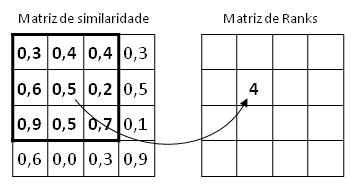
\includegraphics[width=60mm]{conteudo/capitulos/figs/exemplo-matrix-rank-A.png}}
	\subfigure[Passo 2]{\label{fig:b}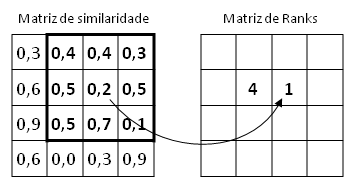
\includegraphics[width=60mm]{conteudo/capitulos/figs/exemplo-matrix-rank-B.png}}
	
	\caption{Exemplo de construção de uma matriz de rankings.%~\cite{Choi2000}.
	}
	\label{fig:exemplomatrixrank}
\end{figure}
% -< Colocar uma explicação mais detalhada para esses passos



Finalmente, com base na matriz de \textit{ranking}, o C99 utiliza um método de \textit{clustering} baseado no algoritmo de maximização de Reynar para identificar os limites entre os segmentos. 
% ~\cite{Reynar1998} 
% Rafael: Esse passo aqui tá meio obscuro ainda. Não dá pra fazer uma figura ilustrativa?




% \subsection{Avaliação}
% \subsubsection{Medidas de Avaliação}


\subsection{Medidas de Avaliação}
% TODO: Escrever um texto sobre acurácia precisição etc...

%  Medidas de avaliação tradicionais 
As medidas de avaliação tradicionais, como acurácia, precisão e revocação, podem não ser confiáveis, por não considerarem a distância entre os limites, mas penalizam o algoritmo sempre que um limite que não coincide perfeitamente com a referência. Essas medidas podem ser mais adequadas quando necessita-se de segmentações com maior exatidão. Em outras palavras, computam apenas os erros do algoritmo quando se detecta falsos positivos ou falsos negativos, o que nesse contexto de segmentação textual pode não ser suficiente, dado a subjetividade da tarefa. Além dessas medidas, que consideram apenas se um segmento foi perfeitamente definido conforme uma referência, pode-se também considerar a distância entre o segmento extraído automaticamente e o segmento de referência~\cite{Kern2009}. Chama-se \textit{near misses} o caso em que um limite identificado automaticamente não coincide exatamente com a referência, mas é necessário considerar a proximidade entre eles.

%  Medidas que consideram a distancia entre os segmentos 
Na Figura~\ref{fig:exemplosegmentacaozoom} é apresentado um exemplo com duas segmentações extraídas automaticamente e uma referência. Em ambos os casos não há nenhum verdadeiro positivo, o que implica em zero para os valores de precisão, acurácia, e revocação, embora o resultado do algoritmo A possa ser considerado superior ao primeiro se levado em conta a proximidade dos limites.
% Para não confundir hipótese com algoritmo, escrever: "A hipótese A, produzida pelo algoritmo A e a hipótese B, produzida pelo algoritmo B".
% Ou trocar hipótese por resultado do algoritmo A, B

  \begin{figure}[!h]

	\centering
	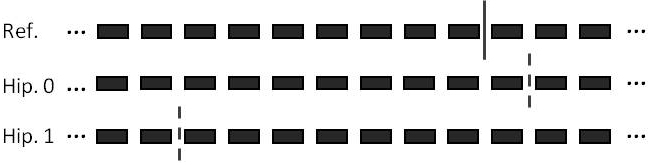
\includegraphics[width=0.6\textwidth]{conteudo/capitulos/figs/windiffzoom.jpg}
	\caption{Exemplos de \textit{near missing} e falso positivo puro. Os blocos indicam uma unidade de informação e as linha verticais representam uma transição de assunto. }
	\label{fig:exemplosegmentacaozoom}

  \end{figure}
  

Considerando o conceito de \textit{near misses}, algumas soluções foram propostas. As medidas de avaliação mais utilizadas são a P$_k$ e \textit{WindowDiff}.
% 
% 
% 
% 
%%%%%%%%%%%%%%%
% Pk 
%%%%%%%%%%%%%%% 
%\item Em~\cite{Beeferman1999} é apresentada uma medida denominada P$_k$, 
% Valores Parciais 
% Funcionamento 
% Compara hipotese e referência		
% Penalisa em caso de discrepânica 
% Calculo de k 
% Medida de dissimilaridade e interpretação 

 
Proposta por~\cite{Beeferman1999}, P$_k$, atribui valores parciais a \textit{near misses}, ou seja, limites sempre receberão um peso proporcional à sua proximidade, desde que dentro de um janela de tamanho~$k$.  Para isso, esse método move uma janela de tamanho $k$ ao longo do texto.  A cada passo verifica, na referência e na hipótese, se o início e o final da janela estão ou não dentro do mesmo segmento, então, penaliza o algoritmo caso não concorde com a referência. Ou seja, dado duas palavras de distância $k$, o algoritmo é penalizado quando não concordar com a segmentação de referência se as palavras estão ou não no mesmo segmento.  O valor de $k$ é calculado como a metade da média dos comprimentos dos segmentos reais. Como resultado, é retornado a contagem de discrepâncias divida pelo quantidade de segmentações analisadas.  P$_k$ é uma medida de dissimilaridade entre as segmentações e pode ser interpretada como a probabilidade de duas sentenças extraídas aleatoriamente pertencerem ao mesmo segmento.  % TODO: Rafael: Não dá pra fazer uma fórmula matemática pra deixar o funcionamento dessa medida mais claro?



%%%%%%%%%%%%%%%
% WindowDiff 
%%%%%%%%%%%%%%% 
%Em \cite{Pevzner2002} 
% Medida alternativa que considera outros aspectos 
% Funcionamento do Windiff 
% Solução para considerar o tamanho das sentenças 
% Solução para equilibrar falsos positivos e near missses 
\textit{WindowDiff} é uma medida alternativa à P$_k$. De maneira semelhante, move uma janela pelo texto e penaliza o algoritmo sempre que o número de limites proposto pelo algoritmo não coincidir com o número de limites esperados para aquela janela. Ou seja, o algoritmo é penalizado quando não concordar com a segmentação de referência quanto ao número de segmentos na janela.  Assim, consegue manter a sensibilidade a \textit{near misses} e além disso, considerar o tamanho das janelas.  A fim de melhor equilibrar o peso dos falsos positivos em relação a \textit{near misses}, dobra-se a penalidade para falsos positivos, evitando-se a supervalorização dessa medida.  % OBS: Os problemas de Pk ficaram subentendidos aqui :/ 

As medidas \textit{WindowDiff} e P$_k$, consideram a quantidade e proximidade entre os limites, sendo mais tolerantes a pequenas imprecisões. Essa é uma característica desejável, visto que as segmentações de referência possuem diferenças consideráveis. \textit{WindowDiff} equilibra melhor os falsos positivos em relação a \textit{near misses}, ao passo que P$_k$ os penaliza com peso maior. Isso significa que segmentadores melhores avaliados em P$_k$ ajudam a selecionar as configurações que erram menos ao separar trechos de texto com o mesmo assunto, enquanto \textit{WindowDiff} é mais tolerante nesse aspecto.  De maneira geral, observa-se  melhores resultados de \textit{WindowDiff} quando os algoritmos aproximam a quantidade de segmentos automáticos da quantidade de segmentos da referência. Por outro lado, P$_K$ avalia melhor as configurações que retornam menos segmentos. Contudo, não é possível definir um valor adequado, uma vez que os segmentadores humanos frequentemente apontam segmentações diferentes.




% --> encerramento da seção de segmentação.
Ao final do processo de segmentação, são produzidos fragmentos de documentos, aqui chamados de subdocumentos. Esses subdocumentos contém um texto, assim como no documento original, em um estágio de processamento inicial, pois ainda não estão estruturados. Ocorre que as técnicas de aprendizado de máquina exigem uma representação estruturada dos textos conforme será visto na Seção~\ref{section:RepTextos}.





